% Source: printed p. 431; PDF p. 440
Nhắc lại khái niệm phức đơn hình (xem Mục~3.4.4.3). Chúng có dạng như sau:
\definecolor{ctsevensimplexblue}{RGB}{95,147,208}
\stepcounter{equation}
\begin{equation}
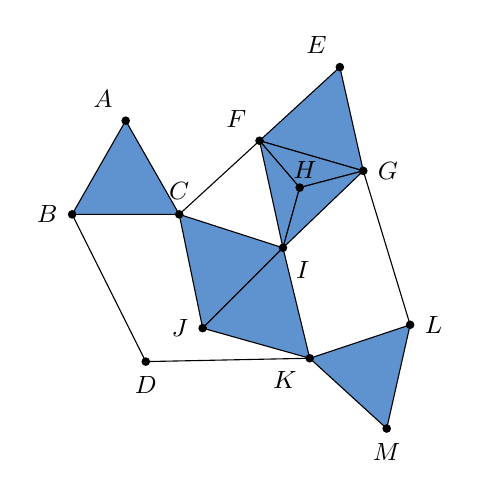
\begin{tikzpicture}[scale=.85,pt/.style={circle,fill,inner sep=1.1pt},font=\small]
\coordinate(A)at(0,3.6);\coordinate(B)at(-.8,2.2);\coordinate(C)at(.8,2.2);\coordinate(D)at(.3,0);
\coordinate(E)at(3.2,4.4);\coordinate(F)at(2,3.3);\coordinate(G)at(3.55,2.85);\coordinate(H)at(2.6,2.6);
\coordinate(I)at(2.35,1.7);\coordinate(J)at(1.15,.5);\coordinate(K)at(2.75,.05);\coordinate(L)at(4.25,.55);\coordinate(M)at(3.9,-1);
\foreach \a/\b/\c in {A/B/C,E/F/G,F/G/H,F/H/I,G/H/I,C/J/I,J/I/K,K/L/M}{\fill[ctsevensimplexblue](\a)--(\b)--(\c)--cycle;\draw(\a)--(\b)--(\c)--cycle;}
\draw(B)--(D)--(K);\draw(C)--(F);\draw(G)--(L);
\foreach \a/\loc in {A/above left,B/left,C/above,D/below,E/above left,F/above left,G/right,I/below right,J/left,K/below left,L/right,M/below}{\node[pt,label=\loc:$\a$]at(\a){};}
\node[pt] at(H){};\node at(2.68,2.86){$H$};
\end{tikzpicture}
\tag{7.10}
\end{equation}
Cho một phức đơn hình $X$ như vậy, ta có thể hình dung mỗi đỉnh $v\in X_0$ là một thực thể có thế giới quan (chẳng hạn một người), và mỗi đơn hình là thế giới quan chung của các đỉnh của nó. Để mô hình hóa điều này, ta gán cho mỗi đỉnh $v\in X$ một olog $\mathcal O(v)$ tương ứng với thế giới quan của thực thể đó; với mỗi đơn hình $u\in X_n$, ta gán một olog $\mathcal O(u)$ tương ứng với một thế giới quan làm nền tảng chung. Nhắc lại rằng $X$ là một tập con của $\mathbb P(X_0)$; nó là một tiền thứ tự và các phần tử của nó (các đơn hình) được sắp thứ tự theo quan hệ bao hàm. Nếu $u,v$ là các đơn hình với $u\subseteq v$, thì ta muốn có một ánh xạ olog (tức là một cấu xạ lược đồ) $\mathcal O(v)\to\mathcal O(u)$. Theo cách này, mô hình nói rằng bất kỳ ý tưởng nào chung cho những người trong $v$ cũng chung cho những người trong $u$. Vậy ta có một hàm tử $\mathcal O:X^{\mathrm{op}}\to\mathbf{Sch}$\ctsevennote{Nguyên bản viết ``$\mathcal O:X\to\mathbf{Sch}$'', nhưng ngay trước đó quy định $u\subseteq v$ cho mũi tên $\mathcal O(v)\to\mathcal O(u)$. Vì thứ tự của $X$ là bao hàm, hàm tử này phải đi từ $X^{\mathrm{op}}$. Đoạn tiếp theo cũng áp dụng $\operatorname{Alx}(X^{\mathrm{op}})$. Bản dịch bổ sung ký hiệu đối để đúng chiều mũi tên.} (ở đây ta bỏ qua sự phân biệt giữa olog và cơ sở dữ liệu để ký hiệu thuận tiện hơn).

Với mỗi phức đơn hình (thực ra với mỗi tập có thứ tự), ta có thể liên kết một không gian tôpô; thực tế, có một hàm tử $\operatorname{Alx}:\mathbf{PrO}\to\mathbf{Top}$, gọi là \emph{hàm tử Alexandrov}. Áp dụng $\operatorname{Alx}(X^{\mathrm{op}})$, ta được một không gian ký hiệu $\mathcal X$. Có thể hình dung $\mathcal X$ như $X$, nhưng các tập mở bao gồm các hợp của những đơn hình. Có một bó các phạm trù duy nhất trên $\mathcal X$ ứng xử như $\mathcal O$ trên các đơn hình của $X$.

\noindent\textit{Ví dụ 7.2.3.12.}\keepwithnext
Hình dung hai nhóm người $G_1$ và $G_2$, mỗi nhóm đưa ra các quan sát về thế giới. Giả sử có một phần giao $H=G_1\cap G_2$. Khi ấy có thể có một cuộc trò chuyện gồm cả $G_1$ và $G_2$, trong đó cả hai nhóm đang nói về cùng một điều (dù dùng những từ khác nhau). $H$ nói: ``Các bạn đang nói về cùng những điều,
% Source: printed p. 432; PDF p. 441
chỉ là dùng những từ khác nhau.'' Trong trường hợp này có một quan sát được đưa ra trên toàn $G_1\cup G_2$, trùng với cả những quan sát trên $G_1$ lẫn những quan sát trên $G_2$.

\subsubsection*{7.2.3.13\quad Thời gian}
Ta có thể dùng bó để mô hình hóa các đối tượng theo thời gian; Goguen~[17] đưa ra một cách tiếp cận. Để có một cách tiếp cận gần hơn với mạch của cuốn sách này, cho $\mathcal C$ là một lược đồ cơ sở dữ liệu. Thời gian tồn tại của thông tin về thế giới nói chung là hữu hạn; nghĩa là điều đúng hôm qua không phải lúc nào cũng đúng hôm nay. Vì vậy, ta có thể gán cho mỗi khoảng thời gian $U$ thông tin mà ta cho là có hiệu lực trên toàn $U$. Đôi khi điều này được gọi là \emph{thời gian hiệu lực của dữ liệu}.

Nếu dữ liệu có hiệu lực trên toàn $U$ và có một tập con $V\subseteq U$, thì dĩ nhiên nó có hiệu lực trên toàn $V$. Điều kiện bó cũng đúng. Nếu một thông tin có hiệu lực trên toàn $U$, và một thông tin khác có hiệu lực trên toàn $V$,\ctsevennote{Nguyên bản viết thông tin thứ hai có hiệu lực ``throughout $U'$'', nhưng sau đó dùng giao $U\cap V$ và hợp $U\cup V$. Bản dịch thống nhất tên của vùng thứ hai là $V$ để các phép hạn chế và ghép dùng đúng hai vùng đã xét.} và nếu hai thông tin này hạn chế thành cùng một thông tin trên giao $U\cap V$, thì ta có thể ghép chúng thành thông tin có hiệu lực trên toàn hợp $U\cup V$.

Vậy ta có thể mô hình hóa sự thay đổi thông tin theo thời gian bằng một bó các $\mathcal C$-tập trên không gian tôpô $\mathbb R$. Nói cách khác, với mỗi khoảng thời gian, ta cho một thể hiện của $\mathcal C$ mà thông tin có hiệu lực trên toàn khoảng ấy. Định nghĩa~7.2.3.5 chỉ định nghĩa bó nhận giá trị trong $\Set$; giờ đây ta tổng quát hóa sang bó trong $\mathcal C\text{--}\Set$. Cụ thể, ta xét các hàm tử $\operatorname{Open}(\mathbb R)^{\mathrm{op}}\to\mathcal C\text{--}\Set$ thỏa cùng điều kiện bó.\ctsevennote{Nguyên bản viết ``$\operatorname{Open}(\mathbb R)\to\mathcal C\text{--}\Set$''. Các ánh xạ hạn chế luôn đi từ thông tin trên vùng lớn đến thông tin trên vùng nhỏ, nên như Định nghĩa~7.2.3.2, miền của hàm tử phải là phạm trù đối $\operatorname{Open}(\mathbb R)^{\mathrm{op}}$.}

\noindent\textit{Ví dụ 7.2.3.14.}\keepwithnext
Xét một bệnh viện nơi các em bé chào đời. Trong tình huống này, các bà mẹ vào bệnh viện, các em bé được sinh ra, rồi mẹ và bé rời bệnh viện. Cho $\mathcal C$ là lược đồ
\begin{center}
\fbox{\begin{tikzpicture}[>=Stealth,font=\small]
\node[draw,label=above:$c$](c)at(0,0){một em bé};
\node[draw,label=above:$m$](m)at(4.8,0){một người mẹ};
\draw[->](c)--node[above]{được sinh bởi}(m);
\end{tikzpicture}}
\end{center}
Xét các khoảng tám giờ
\[
\begin{aligned}
\mathrm{Shift}_1&:=(\text{ngày 1 tháng 1},\ 00{:}00\text{--}08{:}00),\\
\mathrm{Shift}_2&:=(\text{ngày 1 tháng 1},\ 04{:}00\text{--}12{:}00),\\
\mathrm{Shift}_3&:=(\text{ngày 1 tháng 1},\ 08{:}00\text{--}16{:}00).
\end{aligned}
\]
Các y tá làm ca tám giờ, chồng lên ca của người trước bốn giờ; họ chỉ ghi vào cơ sở dữ liệu những bệnh nhân có mặt trong toàn bộ ca của mình hoặc
% Source: printed p. 433; PDF p. 442
trong toàn bộ phần giao giữa các ca. Sau đây là lược đồ:\ctsevennote{Ở ô em bé giao bên phải phía trên, nguyên bản ghi ``$\mathrm{Shift}_1\cap\mathrm{Shift}_3$'', dù các mũi tên đi đến đó xuất phát từ $\mathrm{Shift}_2$ và $\mathrm{Shift}_3$. Các khoảng đã cho có $\mathrm{Shift}_1\cap\mathrm{Shift}_3=\varnothing$, còn giao của ca 2 và ca 3 là khoảng 08:00--12:00. Bản dịch sửa nhãn ô ấy thành $\mathrm{Shift}_2\cap\mathrm{Shift}_3$, phù hợp các mũi tên hạn chế và nhãn vốn đã đúng của ô người mẹ bên dưới.}
\begin{center}
\begin{tikzpicture}[>=Stealth,x=2.55cm,y=1.4cm,font=\scriptsize,box/.style={draw,align=left,inner sep=3pt}]
\node[box](b1)at(0,2){một em bé,\\$\mathrm{Shift}_1$};\node[box](b2)at(1.5,2){một em bé,\\$\mathrm{Shift}_2$};\node[box](b3)at(3,2){một em bé,\\$\mathrm{Shift}_3$};
\node[box](b12)at(.75,3){một em bé,\\$\mathrm{Shift}_1\cap\mathrm{Shift}_2$};\node[box](b23)at(2.25,3){một em bé,\\$\mathrm{Shift}_2\cap\mathrm{Shift}_3$};
\node[box](m1)at(0,0){một người mẹ,\\$\mathrm{Shift}_1$};\node[box](m2)at(1.5,0){một người mẹ,\\$\mathrm{Shift}_2$};\node[box](m3)at(3,0){một người mẹ,\\$\mathrm{Shift}_3$};
\node[box](m12)at(.75,1){một người mẹ,\\$\mathrm{Shift}_1\cap\mathrm{Shift}_2$};\node[box](m23)at(2.25,1){một người mẹ,\\$\mathrm{Shift}_2\cap\mathrm{Shift}_3$};
\foreach\a/\b in {b1/b12,b2/b12,b2/b23,b3/b23,m1/m12,m2/m12,m2/m23,m3/m23,b1/m1,b3/m3,b12/m12,b23/m23}{\draw[->](\a)--(\b);}
\draw[->](b2)--node[pos=.25,right]{được sinh bởi}(m2);
\end{tikzpicture}
\end{center}
Chắc chắn còn có thể bàn luận liệu cách triển khai ngữ nghĩa bó này có hữu ích nhất trong thực tế hay không. Nhưng một cách nào đó tương tự có thể dễ dàng hữu ích như một ngữ nghĩa, tức một cách suy nghĩ về bản chất thời gian của dữ liệu.

\section{Monad}
Có lẽ monad đã không được phát minh nếu không có lý thuyết phạm trù, nhưng chúng đã tỏ ra hữu ích để hiểu các lý thuyết đại số, tính các bất biến của không gian tôpô và đưa những phép toán không mang tính hàm vào các ngôn ngữ lập trình hàm. Ta chủ yếu bàn về monad theo cách chúng giúp làm rõ một bối cảnh mô hình hóa đã cho, qua đó cho phép đơn giản hóa ngôn ngữ dùng trong các mô hình ấy. Ta dùng cơ sở dữ liệu để đưa ra các ví dụ cụ thể.

Phần lớn nội dung về monad dưới đây được lấy từ Spivak~[40].

\subsection{Monad hình thức hóa bối cảnh}
Monad có thể hình thức hóa các giả định về cách ta làm việc trong toàn bộ một lĩnh vực. Chẳng hạn, giả sử ta muốn xét những hàm không bắt buộc phải trả về một
% Source: printed p. 434; PDF p. 443
giá trị cho mọi đầu vào. Đây không phải là các hàm hợp lệ theo định nghĩa ở Mục~2.1.2 (vì chúng không toàn phần), nhưng trong các lớp toán, ta muốn nói về $f(x)=\frac1x$ và $g(x)=\tan(x)$ như thể chúng là các hàm $\mathbb R\to\mathbb R$, để có thể hợp thành chúng mà không phải liên tục chú ý đến miền xác định.

Những hàm không bắt buộc phải được định nghĩa trên toàn bộ miền của mình được gọi là \emph{hàm bộ phận}. Ai cũng biết chúng nên hoạt động ra sao, nên ta cần một cách làm cho điều đó hợp lệ về mặt toán học. Monad và các \emph{phạm trù Kleisli} mà chúng sinh ra cho ta một cách thực hiện việc này. Cụ thể, ta sẽ có thể bàn một cách hình thức về hợp thành
\[
\mathbb R\xrightarrow{\frac1x}\mathbb R\xrightarrow{\tan(x)}\mathbb R.
\]
Ở đây ta vẽ các mũi tên giữa những tập hợp như thể đang nói về hàm toàn phần, nhưng có một bối cảnh ngầm trong đó ta thực sự nói về hàm bộ phận. Monad cho phép ta viết các ánh xạ giữa tập hợp theo lối hàm, trong khi vẫn giữ bối cảnh nền. Điều khiến chúng hữu ích là khái niệm \emph{bối cảnh} đang dùng ở đây được làm cho hình thức.

\noindent\textit{Ví dụ 7.3.1.1 (Hàm bộ phận).}\keepwithnext
Có thể mô hình hóa hàm bộ phận bằng hàm thông thường nếu ta thêm một phần tử đặc biệt ``không có câu trả lời'' vào đối miền. Nghĩa là tập các hàm bộ phận $A\to B$ tương ứng một-một với tập các hàm thông thường $A\to B\sqcup\{\ctsevensmiley\}$. Chẳng hạn, giả sử ta muốn mô hình hóa hàm bộ phận $f_p(x):=\frac1{x^2-1}:\mathbb R\to\mathbb R$ theo cách này; ta dùng hàm toàn phần $f_t:\mathbb R\to\mathbb R\sqcup\{\ctsevensmiley\}$, định nghĩa bởi:
\[
f(x):=\begin{cases}
\dfrac1{x^2-1}&\text{nếu }x\ne-1\text{ và }x\ne1,\\
\ctsevensmiley&\text{nếu }x=-1,\\
\ctsevensmiley&\text{nếu }x=1.
\end{cases}
\]
Một hàm thông thường $g:A\to B$ có thể được coi là một hàm bộ phận vì ta có thể hợp thành nó với phép bao hàm
\stepcounter{equation}
\begin{equation}
B\longrightarrow B\sqcup\{\ctsevensmiley\}.
\tag{7.11}
\end{equation}
để được $A\to B\sqcup\{\ctsevensmiley\}$.

Nhưng ta hợp thành hai hàm bộ phận được viết theo cách này ra sao? Giả sử $f:A\to B\sqcup\{\ctsevensmiley\}$ và $g:B\to C\sqcup\{\ctsevensmiley\}$ là các hàm. Trước hết tạo một hàm mới
\[
g':=g\sqcup\{\ctsevensmiley\}:B\sqcup\{\ctsevensmiley\}\longrightarrow C\sqcup\{\ctsevensmiley\}\sqcup\{\ctsevensmiley\},
\]
rồi hợp thành để được $(g'\circ f):A\to C\sqcup\{\ctsevensmiley\}\sqcup\{\ctsevensmiley\}$; cuối cùng gửi cả hai $\ctsevensmiley$ đến cùng một phần tử bằng cách hợp thành với
\stepcounter{equation}
\begin{equation}
C\sqcup\{\ctsevensmiley\}\sqcup\{\ctsevensmiley\}\longrightarrow C\sqcup\{\ctsevensmiley\}.
\tag{7.12}
\end{equation}

% Source: printed p. 435; PDF p. 444
Ta nên hiểu phép hợp thành các hàm bộ phận $g\circ f$ như thế nào? Mỗi phần tử $a\in A$ được $f$ gửi đến một phần tử $b\in B$ hoặc đến ``không có câu trả lời''. Nếu nó có một câu trả lời $f(a)\in B$, thì câu trả lời ấy lại được $g$ gửi đến một phần tử $g(f(a))\in C$ hoặc đến ``không có câu trả lời''. Ta được một hàm bộ phận $A\to C$ bằng cách gửi $a$ đến $g(f(a))$ nếu có thể, hoặc đến ``không có câu trả lời'' nếu nó bị dừng ở một bước nào đó.

Trong khoa học máy tính, monad này đôi khi được gọi là \emph{monad maybe}, vì một hàm bộ phận $f:A\to B$ nhận mỗi phần tử của $A$ và có thể xuất ra một phần tử của $B$, hoặc có thể không xuất ra gì; nói gọn hơn, nó xuất ra một ``maybe $B$'' (có thể có một $B$).

\noindent\textit{Bài tập 7.3.1.2.}\keepwithnext
\begin{enumerate}[label=\alph*.]
\item Cho $f:\mathbb Z\to\mathbb Q\sqcup\{\ctsevensmiley\}$ là hàm bộ phận cho bởi $f(n)=\frac1{n^2-n}$.\ctsevennote{Nguyên bản khai báo ``$f:\mathbb Z\to\mathbb Z\sqcup\{\ctsevensmiley\}$'', và cả hai bảng lời giải cũng ghi đối miền $\mathbb Z\sqcup\{\ctsevensmiley\}$. Nhưng các giá trị được yêu cầu và được tác giả tính, như $f(-3)=1/12$, không phải số nguyên. Bản dịch dùng $\mathbb Q\sqcup\{\ctsevensmiley\}$ làm đối miền cho $f$ và $f\circ g$, giữ nguyên mọi công thức và giá trị; $g$ vẫn nhận giá trị nguyên khi xác định.} Tính các giá trị sau: $f(-3)$, $f(-2)$, $f(-1)$, $f(0)$, $f(1)$ và $f(2)$.
\item Cho $g:\mathbb Z\to\mathbb Z\sqcup\{\ctsevensmiley\}$ là hàm bộ phận cho bởi
\[
g(n)=\begin{cases}n^2-3&\text{nếu }n\ge-1,\\\ctsevensmiley&\text{nếu }n<-1.\end{cases}
\]
Viết $f\circ g(n)$ với $-3\le n\le2$.
\nobreak\hfill$\diamond$
\end{enumerate}

\noindent\textit{Lời giải 7.3.1.2.}\keepwithnext
\begingroup\renewcommand{\arraystretch}{1.5}
\[
\text{a. }\begin{array}{|c||c|}\hline\multicolumn{2}{|c|}{f}\\\hline\mathbb Z&\mathbb Q\sqcup\{\ctsevensmiley\}\\\hline
-3&\frac1{12}\\\hline-2&\frac16\\\hline-1&\frac12\\\hline0&\ctsevensmiley\\\hline1&\ctsevensmiley\\\hline2&\frac12\\\hline\end{array}
\qquad
\text{b. }\begin{array}{|c||c|}\hline\multicolumn{2}{|c|}{f\circ g}\\\hline\mathbb Z&\mathbb Q\sqcup\{\ctsevensmiley\}\\\hline
-3&\ctsevensmiley\\\hline-2&\ctsevensmiley\\\hline-1&\frac16\\\hline0&\frac1{12}\\\hline1&\frac16\\\hline2&\ctsevensmiley\\\hline\end{array}
\]
\nobreak\hfill$\blacklozenge$\par
\endgroup

\noindent\textit{Ứng dụng 7.3.1.3.}\keepwithnext
Các thí nghiệm phải được thực hiện khách quan, nhưng giả sử ta hình dung rằng việc thay người làm thí nghiệm, chẳng hạn trong tâm lý học,
% Source: printed p. 436; PDF p. 445
có thể làm thay đổi kết quả. Cho $A$ là tập những người làm thí nghiệm, $X$ là không gian tham số của các biến thí nghiệm (chẳng hạn $X=\text{Tuổi}\times\text{Thu nhập}$), và $Y$ là không gian quan sát (chẳng hạn $Y=\text{xu hướng bạo lực}$). Ta muốn hiểu một thí nghiệm như vậy là cho biết về một hàm $f:X\to Y$ (tuổi và thu nhập ảnh hưởng thế nào đến xu hướng bạo lực). Tuy nhiên, ta có thể muốn làm rõ một phần bối cảnh bằng cách đưa vào thông tin về người đã thực hiện thí nghiệm. Nghĩa là ta thực sự đang tìm một hàm $f:X\times A\to Y$.

Cho một tập người $P$, người làm thí nghiệm muốn biết tuổi và thu nhập của từng người, tức một hàm $P\to X$. Tuy nhiên, có thể ngay cả việc xác định thông tin cơ bản này, chỉ bằng cách hỏi mỗi người các câu hỏi ấy, cũng phụ thuộc vào người làm thí nghiệm nào trong $A$ đang hỏi. Khi đó ta lại muốn xem người làm thí nghiệm là một phần của bài toán, thay hàm $P\to X$ bằng một hàm $P\times A\to X$. Trong trường hợp như vậy, ta có thể dùng một monad để ẩn sự kiện rằng mọi thứ đang xét đều được giả định chịu ảnh hưởng của $A$. Nói cách khác, ta muốn công bố một lần cho tất cả bối cảnh mô hình hóa---rằng mọi đại lượng quan sát có thể chịu ảnh hưởng của người quan sát---để sau đó nó có thể lùi vào nền.

Ta sẽ quay lại điều này trong các Ví dụ~7.3.2.6 và~7.3.3.4.
\hfill$\diamond\diamond$

\subsection{Định nghĩa và ví dụ}
Những khía cạnh nào của Ví dụ~7.3.1.1 nói về monad, và những khía cạnh nào nói riêng về hàm bộ phận? Monad là những cấu trúc gồm một hàm tử và một vài biến đổi tự nhiên. Nói sơ lược, hàm tử cho hàm bộ phận là $B\mapsto B\sqcup\{\ctsevensmiley\}$, và các biến đổi tự nhiên được cho trong~(7.11) và~(7.12). Mục này đưa ra định nghĩa monad cùng vài ví dụ. Ở Mục~7.3.3, ta quay lại xem monad hình thức hóa bối cảnh như thế nào.

\noindent\textbf{Định nghĩa 7.3.2.1 (Monad).}\keepwithnext
Một \emph{monad trên $\Set$} được định nghĩa như sau: ta công bố một số thành phần (A. hàm tử, B. ánh xạ đơn vị, C. ánh xạ nhân) và chứng minh rằng chúng tuân theo một số luật (1. các luật đơn vị, 2. luật kết hợp). Cụ thể, ta công bố
\begin{enumerate}[label=\Alph*.]
\item một hàm tử $T:\Set\to\Set$,
\item một biến đổi tự nhiên $\eta:\id_{\Set}\to T$,
\item một biến đổi tự nhiên $\mu:T\circ T\to T$.
\end{enumerate}
Đôi khi ta nói về hàm tử $T$ như thể nó là toàn bộ monad; ta gọi $\eta$ là \emph{ánh xạ đơn vị} và $\mu$ là \emph{ánh xạ nhân}. Sau đó phải chứng minh các \emph{luật monad} sau đúng:
% Source: printed p. 437; PDF p. 446
\begin{enumerate}[label=\arabic*.]
\item Các sơ đồ hàm tử $\Set\to\Set$ sau giao hoán:
\[
\begin{tikzcd}[column sep=large,row sep=large]
T\circ\id_{\Set}\arrow[r,"\id_T\diamond\eta"]\arrow[dr,"="']&T\circ T\arrow[d,"\mu"]\\&T
\end{tikzcd}\qquad
\begin{tikzcd}[column sep=large,row sep=large]
\id_{\Set}\circ T\arrow[r,"\eta\diamond\id_T"]\arrow[dr,"="']&T\circ T\arrow[d,"\mu"]\\&T
\end{tikzcd}
\]
\item Sơ đồ hàm tử $\Set\to\Set$ sau giao hoán:
\[
\begin{tikzcd}[column sep=large,row sep=large]
T\circ T\circ T\arrow[r,"\mu\diamond\id_T"]\arrow[d,"\id_T\diamond\mu"']&T\circ T\arrow[d,"\mu"]\\
T\circ T\arrow[r,"\mu"']&T
\end{tikzcd}
\]
\end{enumerate}

\noindent\textit{Ví dụ 7.3.2.2 (Monad List).}\keepwithnext
Bây giờ ta đi qua Định nghĩa~7.3.2.1 với monad $\operatorname{List}$. Bước đầu tiên là cho một hàm tử $\operatorname{List}:\Set\to\Set$, như đã làm trong Ví dụ~5.1.2.20. Nhắc lại rằng nếu $X=\{p,q,r\}$, thì $\operatorname{List}(X)$ gồm danh sách rỗng $[\,]$, những danh sách một phần tử như $[p]$, và mọi danh sách khác của các phần tử trong $X$, chẳng hạn $[p,p,r,q,p]$. Cho một hàm $f:X\to Y$, ta được một hàm $\operatorname{List}(f):\operatorname{List}(X)\to\operatorname{List}(Y)$ bằng cách áp dụng $f$ lên từng phần tử, như trong Bài tập~5.1.2.22.

Là một monad, hàm tử $\operatorname{List}$ đi kèm hai biến đổi tự nhiên: một ánh xạ đơn vị $\eta$ và một ánh xạ nhân $\mu$. Cho một tập $X$, ánh xạ đơn vị $\eta_X:X\to\operatorname{List}(X)$ trả về các danh sách một phần tử như sau:
\[
\begin{array}{rcl}
X&\xrightarrow{\eta_X}&\operatorname{List}(X)\\\hline
p&\longmapsto&[p]\\q&\longmapsto&[q]\\r&\longmapsto&[r]
\end{array}
\]
Cho một tập $X$, ánh xạ nhân $\mu_X:\operatorname{List}(\operatorname{List}(X))\to\operatorname{List}(X)$ nối các danh sách
% Source: printed p. 438; PDF p. 447
của danh sách như sau:
\[
\begin{array}{rcl}
\operatorname{List}(\operatorname{List}(X))&\xrightarrow{\mu_X}&\operatorname{List}(X)\\\hline
{}[[p],[q]]&\longmapsto&[p,q]\\
{}[[q,p,r],[\,],[q,r,p,r],[r]]&\longmapsto&[q,p,r,q,r,p,r,r]
\end{array}
\]
Tính tự nhiên của $\eta$ và $\mu$ có nghĩa là các ánh xạ này hoạt động phù hợp khi ta áp dụng một hàm $f:X\to Y$ lên từng phần tử. Cuối cùng, có thể minh họa ba luật monad trong Định nghĩa~7.3.2.1 như sau:\ctsevennote{Trong các sơ đồ minh họa này, nguyên bản ghi $\id_{\operatorname{List}}\circ\eta$, $\eta\circ\id_{\operatorname{List}}$, $\mu\circ\id_{\operatorname{List}}$ và $\id_{\operatorname{List}}\circ\mu$. Chúng biểu thị phép hợp thành ngang (ghép bên) của các biến đổi tự nhiên, nên bản dịch viết $\diamond$ nhất quán với các sơ đồ tổng quát trong Định nghĩa~7.3.2.1.}
\[
\begin{tikzcd}[column sep=large,row sep=large]
{[p,q,q]}\arrow[r,mapsto,"\id_{\operatorname{List}}\diamond\eta"]\arrow[dr,equal]&{[[p],[q],[q]]}\arrow[d,mapsto,"\mu"]\\&{[p,q,q]}
\end{tikzcd}\qquad
\begin{tikzcd}[column sep=large,row sep=large]
{[p,q,q]}\arrow[r,mapsto,"\eta\diamond\id_{\operatorname{List}}"]\arrow[dr,equal]&{[[p,q,q]]}\arrow[d,mapsto,"\mu"]\\&{[p,q,q]}
\end{tikzcd}
\]
\[
\begin{tikzcd}[column sep=small,row sep=large,font=\scriptsize]
{\bigl[[[p,q],[r,r]],[[\,],[r,q,q]]\bigr]}\arrow[r,mapsto,"\mu\diamond\id_{\operatorname{List}}"]\arrow[d,mapsto,"\id_{\operatorname{List}}\diamond\mu"']&{\bigl[[p,q],[r,r],[\,],[r,q,q]\bigr]}\arrow[d,mapsto,"\mu"]\\
{\bigl[[p,q,r,r],[r,q,q]\bigr]}\arrow[r,mapsto,"\mu"']&{[p,q,r,r,r,q,q]}
\end{tikzcd}
\]

\noindent\textit{Bài tập 7.3.2.3.}\keepwithnext
Cho $\mathbb P:\Set\to\Set$ là hàm tử tập lũy thừa, sao cho với một hàm $f:X\to Y$, hàm $\mathbb P(f):\mathbb P(X)\to\mathbb P(Y)$ được cho bằng cách lấy ảnh.
\begin{enumerate}[label=\alph*.]
\item Hiểu phát biểu: ``Với $\eta$ được định nghĩa bằng các tập con một phần tử và $\mu$ được định nghĩa bằng phép hợp, $\top:=(\mathbb P,\eta,\mu)$ là một monad.''
\item Với $X=\{a,b\}$, viết hàm $\eta_X$ dưới dạng một bảng hai hàng, hai cột.
\item Với $X=\{a,b\}$, viết hàm $\mu_X$ dưới dạng một bảng mười sáu hàng, hai cột (bạn có thể dừng sau năm hàng nếu đã hiểu đầy đủ).
\item Kiểm tra để tin rằng các luật monad trong Định nghĩa~7.3.2.1 đúng.
\nobreak\hfill$\diamond$
\end{enumerate}
